
%\documentclass[calculator,allquestions,datasheet,solutions]{exam_newMarcus2}
%\documentclass[calculator,allquestions,datasheet,resit]{exam_newMarcus2}
\documentclass[calculator,steamtables,allquestions,datasheet,resit,solution]{exam_newMarcus2}

% The full list of class options are
% calculator : Allows approved calculator use.
% datasheet : Adds a note that data sheet are attached to the exam.
% handbook : Allows the use of the engineering handbook.
% resit : Adds the resit markings to the paper.
% sample : Adds conspicuous SAMPLE markings to the paper
% solutions : Uses the contents of \solution commands (and \solmarks) to generate a solution file

\usepackage{pdfpages}   
\usepackage{lscape,comment}
 
\coursecode{EX3029}%%
\coursetitle{Chemical Thermodynamics}
 
\examtime{09.00--12.00}%
\examdate{03}{06}{2017}% 
\examformat{Candidates must attempt \textit{all} questions, each of which carries equal (20) marks.  All thermodynamic symbols have their usual meanings unless otherwise stated.}

\newcommand{\frc}{\displaystyle\frac}
\newcommand{\br}[1]{\!\left( #1 \right)}
\newcommand{\abs}[1]{\left| #1 \right|}
\newcommand{\fracd}[2]{\frac{\mathrm{d} #1}{\mathrm{d} #2}}
\newcommand{\fracp}[2]{\frac{\partial #1}{\partial #2}}
\renewcommand{\d}[1]{\mathrm{d} #1 } 
\newcommand{\Ma}{\mathrm{M\!a}} 



\begin{document}


%%%
%%% Question 02
%%%
\begin{question}
\begin{enumerate}[(a)]
%
\item Derive the Maxwell relations below from the fundamental thermodynamic equations.~\marks{11}
\begin{eqnarray}
 \left(\frac{\partial T}{\partial V}\right)_{S} = -\left(\frc{\partial P}{\partial S}\right)_{V}; && 
 \left(\frc{\partial T}{\partial P}\right)_{S} = \left(\frac{\partial V}{\partial S}\right)_{P}; \nonumber \\
 \left(\frc{\partial P}{\partial T}\right)_{V} = \left(\frac{\partial S}{\partial V}\right)_{T}; &&%
  \left(\frac{\partial V}{\partial T}\right)_{P} = -\left(\frc{\partial S}{\partial P}\right)_{T} \nonumber 
\end{eqnarray}
%==========================
%
\solution{First, let's assume a functional $f=f\left(a,b\right)$ and rewrite it as a function of the variables $a$ and $b$,~\solmarks{1/11}
\begin{displaymath}
df = \left(\frc{\partial f}{\partial a}\right)_{b}da + \left(\frc{\partial f}{\partial b}\right)_{a}db
\end{displaymath}
If we define $M=\left(\frc{\partial f}{\partial a}\right)_{b}$ and $N=\left(\frc{\partial f}{\partial b}\right)_{a}$, the equation above becomes~\solmarks{1/11}
\begin{equation}
{\bf df = M da + N db}\label{eqn1}
\end{equation}
Now, if we differentiate $M$ and $N$ with respect to $b$ and $a$, respectively,~\solmarks{1/11}
\begin{displaymath}
\left(\frc{\partial M}{\partial b}\right)_{a} = \frc{\partial^{2} f}{\partial a\partial b}\;\;\text{ and }\;\;\left(\frc{\partial N}{\partial a}\right)_{b} = \frc{\partial^{2} f}{\partial b\partial a}
\end{displaymath}
If the functional $f$ is continuous and differentiable over all domain,~\solmarks{1/11}
\begin{equation}\label{eqn2}
\frc{\partial^{2} f}{\partial a\partial b} = \frc{\partial^{2} f}{\partial b\partial a} \Longrightarrow {\bf \left(\frc{\partial M}{\partial b}\right)_{a} = \left(\frc{\partial N}{\partial a}\right)_{b} }
\end{equation}
The fundamental thermodynamic relations,~\solmarks{1/11} 
\begin{eqnarray}
&& dU = - PdV + TdS \nonumber \\ 
&& dH =   TdS + VdP \nonumber \\
&& dA = - PdV - SdT \nonumber \\
&& dG = - VdP - SdT \nonumber
\end{eqnarray}
have similar shape as Eqn.~\ref{eqn1}, where, for example, in the first relation: ~\solmarks{1/11} 
   \begin{displaymath}
     U = f,\; M=-P,\; N=T,\; \d V=\d a\;\text{ and }\; \d S=\d b. 
   \end{displaymath}
Using relation~\ref{eqn2},~\solmarks{2/11}
   \begin{displaymath}
         -\left(\frc{\partial P}{\partial S}\right)_{V}=\left(\frc{\partial T}{\partial V}\right)_{S}.
   \end{displaymath}
Applying the same to the remaining relations we obtain:~\solmarks{3/11}
\begin{displaymath}
 \left(\frc{\partial T}{\partial P}\right)_{S} = \left(\frac{\partial V}{\partial S}\right)_{P},\; \left(\frc{\partial P}{\partial T}\right)_{V} = \left(\frac{\partial S}{\partial V}\right)_{T}, \text{ and }\; \left(\frac{\partial V}{\partial T}\right)_{P} = -\left(\frc{\partial S}{\partial P}\right)_{T} 
\end{displaymath}
}
%
\item Using the Maxwell relations above, evaluate $\left(\frc{\partial S}{\partial V}\right)_{T}$ for water vapour at 240$^{\circ}$C and molar volume of 0.0258 m$^{3}$ mol$^{-1}$ through the Redlich-Kwong equation of state,
\begin{displaymath}
P = \frc{RT}{V-b} - \frc{a}{V\left(V+b\right)T^{1/2}}
\end{displaymath}
with 
$R$ = 8.314$\times$ 10$^{-5}\;\text{bar m}^{3} \left(\text{mol K}\right)^{-1}$, $a$ = 142.59 $\times$ 10$^{-6}\;\text{bar m}^{6} \left(\text{mol K}\right)^{-2}$ and $b$ = 0.0211 $\times$ 10$^{-3}\text{m}^{3}\;\text{mol}^{-1}$.~\marks{9}


%\frc{\text{bar.m}^{3}}{\text{mol.K}}$, $a$ = 142.59 $\times$ 10$^{-6}\; \frc{\text{bar.m}^{6}}{\left(\text{mol.K}\right)^{2}}$ and $b$ = 0.0211 $\times$ 10$^{-3}\frc{\text{m}^{3}}{\text{mol}}$.~\marks{9}
%==========================
\solution{The Maxwell relation ~\solmarks{2/9}
   \begin{displaymath}
      \left(\frc{\partial P}{\partial T}\right)_{V} = \left(\frc{\partial S}{\partial V}\right)_{T}
   \end{displaymath}
    allows to determine $\left(\frc{\partial S}{\partial V}\right)_{T}$ from the PVT relationship in the RK EOS. Thus,~\solmarks{4/9}
\begin{displaymath}
{\bf \left(\frc{\partial P}{\partial T}\right)_{V} = \frc{R}{V-b} + \frc{a}{2 V\left( V + b \right)T^{\frac{3}{2}}}}
\end{displaymath}
Now substituting the variables by their values~\solmarks{3/9}
\begin{displaymath}
  \left(\frc{\partial P}{\partial T}\right)_{V} = \left(\frc{\partial S}{\partial V}\right)_{T} = 3.2342\times 10^{-3} \text{bar.K}^{-1} = 3.2342\times 10^{-1}\frc{\text{kJ}}{\text{m}^{3}.\text{K}}
\end{displaymath}

}
%
\end{enumerate}
\end{question}
\clearpage



%%%
%%% Question 01
%%%
\begin{question}
%
\begin{enumerate}[(a)] % (Shapiro 2.34) 
\item A closed system with 0.09 kg of air undergoes a polytropic process from P$_{1}$ = 138 kPa, v$_{1}$ = 0.72 m$^{3}$ kg$^{-1}$ to a final state where P$_{2}$ = 552 kPa, v$_{2}$ = 0.25 m$^{3}$ kg$^{-1}$.  Determine the work (in kJ) required for this compression.~\marks{8} 
\solution{
First stage is to calculate the polytropic coefficient,
\begin{displaymath}
P_{1}v_{1}^{n} = P_{2}v_{2}^{n} \Longrightarrow {\bf n} = \frc{\ln P_{2}/P_{1}}{\ln v_{1}/v_{2}} {\bf = 1.31}
\end{displaymath}~\solmarks{4/8}
Now, calculating the work with $V_{i}=v_{i}\times m$, thus V$_{1}=0.0648$ m$^{3}$ and V$_{2}=0.0225$ m$^{3}$:
\begin{eqnarray}
{\bf W }&=& -\int\limits_{V_{1}}^{V_{2}} P dV = -\int\limits_{V_{1}}^{V_{2}} \frc{C}{V^{n}} dV = -\left.C \frc{V^{1-n}}{1-n}\right|_{V_{1}}^{V_{2}} = -\frc{P_{2}V_{2}^{n}V_{2}^{1-n}-P_{1}V_{1}^{n}V_{1}^{1-n}}{1-n} = -\frc{P_{2}V_{2}-P_{1}V_{1}}{1-n} \nonumber \\
   &=& {\bf 11.214 kJ} \nonumber
\end{eqnarray} ~\solmarks{4/8}}



\item Calculate the compressibility factor ($Z$) of chloroform vapour at 450 K and 20 bar (molar volume of 1.35$\times$10$\left.^{-3}\text{ m}^{3}\;\text{mol}^{-1}\right)$ using the Soave-Redlich-Kwong equation of state. If you are using an iterative method (i.e., hand-calculation), do use the ideal gas equation of state to estimate the initial guess, $Z_{0}$, and stop at the second iteration, $Z_{2}$. Properties of chloroform are: T$_{c}$ = 537 K, P$_{c}$ = 5328.68 kPa and $\omega$ = 0.218 (accentric factor).~\marks{12}
\solution{ The generic form of $Z$ is,
\begin{displaymath}
Z = 1+ \beta - q\beta\frc{Z - \beta}{\left(Z+\epsilon\beta\right)\left(Z+\sigma\beta\right)}\;\;\text{ with} \;\; \beta = \Omega \frc{P_{r}}{T_{r}}\;\;\text{ and}\;\; q=\frc{\Psi\alpha}{\Omega T_{r}}
\end{displaymath}
For SRK with {\bf T$_{r}$=0.8380}, {\bf P$_{r}$=0.3754}, {\bf $\beta$=3.88$\times$10$^{-2}$} and {\bf $q$=6.7274}~\solmarks{2/12},
\begin{displaymath}
{\bf Z = 1 + \beta - q\beta\frc{Z-\beta}{Z^{2}+\beta Z}}
\end{displaymath}~\solmarks{2/12}
The equation is non-linear and to find the root we can apply Newton-Raphson method 
\begin{displaymath}
Z_{i} = Z_{i-1} - \frc{\mathcal{F}\left(Z_{i-1}\right)}{d\mathcal{F}/dZ \left(Z_{i-1}\right)}
\end{displaymath}
with,
\begin{eqnarray}
&& \mathcal{F}\left(Z\right) = Z - \left[ 1 + \beta - q\beta\frc{Z-\beta}{Z^{2}+\beta Z}\right] \nonumber \\
&& \frc{d\mathcal{F}}{dZ}\left(Z\right) = 1 + q\beta \frc{\beta^{2}+2\beta Z- Z^{2}}{\left(Z^{2}+\beta Z\right)^{2}} \nonumber
%\frc{q\beta\left(Z^{2}\beta +Z\right)-q\beta Z\left(2Z + \beta\right)}{\left(Z^{2}+\beta Z\right)^{2}} + \frc{q\beta^{2}\left(2Z+\beta\right)}{\left(Z^{2}+\beta Z\right)^{2}} \nonumber
\end{eqnarray} 
%as initial guess, we can use the generic real gas EOS, $PV=Z_{0}RT \Longrightarrow$ $Z_{0}=0.7217$. Thus 
\begin{center}
{\bf $Z_{1}$ = 0.7184}~\solmarks{4/12} \\
{\bf $Z_{2}$ = 0.7160}~\solmarks{4/12} \\
$\cdots \cdots \cdots $ \\
\textcolor{red} {or (using calculator) }{\bf $Z_{22}$ = 0.7088}~\solmarks{\textcolor{red}{10/12}} \\

\end{center}
} 

\end{enumerate}

\end{question} 
\clearpage


%%%
%%% Question 01
%%%
\begin{question}
%
%%%
%%% Jeff Solved Example 3 ==> Sandler Example 10.1.4 (page 504)
%%%
 An ideal liquid mixture of 25 mol$\%$ n-pentane $\left(nC_{5}\right)$, 45 mol$\%$ n-hexane $\left(nC_{6}\right)$ and 30 mol$\%$ n-heptane $\left(nC_{7}\right)$, initially at 69$^{\circ}$C and high pressure, is partially vaporised by isothermically lowering the pressure to 1.013 bar. Calculate:
\begin{enumerate}[(a)]
%
   \item Saturation pressure, P$_{i}^{\text{sat}}$, of n-pentane, n-hexane and n-heptane (in bar).~\marks{3}
%======================
         \solution{ From the Antoine equation, we can calculate the saturation pressure of the species $P_{\text{C}_{5}}^{sat}=$ 2.721 bar, $P_{\text{C}_{6}}^{sat}=$ 1.024 bar and $P_{\text{C}_{7}}^{sat}=$ 0.389 bar.~\solmarks{3/3}
}
%
   \item Vapour-liquid equilibrium constant $\left(K_{i}=y_{i}.x_{i}^{-1}\right.$ where $x_{i}$ and $y_{i}$ are molar fractions of liquid and vapour phases, respectively$\left.\right)$ of all components.~\marks{6}
%======================
         \solution{  Assuming ideal solution,
\begin{displaymath}
K_{i} = \frc{y_{i}}{x_{i}} = \frc{P_{i}^{sat}}{P}
\end{displaymath}
Thus $K_{\text{C}_{5}}=$ 2.6861, $K_{\text{C}_{6}}=$ 1.0109 and $K_{\text{C}_{7}}=$ 0.3840~\solmarks{6/6}
}
%
   \item Relative amounts of vapour and liquid (i.e., molar fractions of phases $V$ and $L$) in equilibrium and their compositions $\left(x_{i}\text{ and } y_{i}\right)$.~\marks{11}
%======================
         \solution{ From $K_{i} = \frc{y_{i}}{x_{i}}$,
\begin{eqnarray}
&& y_{\text{C}_{5}} = x_{\text{C}_{5}}K_{\text{C}_{5}},\;\; y_{\text{C}_{6}} = x_{\text{C}_{6}}K_{\text{C}_{6}},\;\; y_{\text{C}_{7}} = x_{\text{C}_{7}}K_{\text{C}_{7}} \nonumber \\
&& \sum\limits_{i=1}^{3}x_{i} = x_{\text{C}_{5}} + x_{\text{C}_{6}} + x_{\text{C}_{7}} = 1  \nonumber \\
&& \sum\limits_{i=1}^{3}y_{i} = y_{\text{C}_{5}} + y_{\text{C}_{6}} + y_{\text{C}_{7}} = 1  = K_{\text{C}_{5}}x_{\text{C}_{5}} + K_{\text{C}_{6}}x_{\text{C}_{6}} + K_{\text{C}_{7}}x_{\text{C}_{7}} \nonumber
\end{eqnarray}
The mass balance is,~\solmarks{1/11}
\begin{eqnarray}
&& L + V = 1 \nonumber \\
&& x_{i}L + y_{i}V = z_{i} \nonumber 
\end{eqnarray}
with $z_{i}=\left(0.25\;\;0.45\;\;0.30\right)^{T}$. Rearranging this set of equations lead to a non-linear expression in $L$,~\solmarks{2/11}
\begin{displaymath}
\frc{0.25}{\left(1-K_{\text{C}_{5}}\right)L+K_{\text{C}_{5}}} + \frc{0.45}{\left(1-K_{\text{C}_{6}}\right)L+K_{\text{C}_{6}}} +  \frc{0.30}{\left(1-K_{\text{C}_{7}}\right)L+K_{\text{C}_{7}}} = 1 
\end{displaymath}
Solving this equation leads to $L=0.5748$ and $V=0.4252$~\solmarks{2/11}. Calculating the molar fractions of the species:~\solmarks{6/11}
\begin{center}
\begin{tabular}{c c c c}
\hline
                 & {\bf n-C$_{5}$} &  {\bf n-C$_{6}$} &  {\bf n-C$_{7}$} \\
\hline
  {\bf x$_{i}$}   & 0.1456         &  0.4479         & 0.4065    \\
  {\bf y$_{i}$}   &  0.3911        &  0.4528         & 0.1561    \\
\hline
\end{tabular} 
\end{center}}

%
\end{enumerate}

For this problem, use 
\begin{displaymath}
   \ln P_{i}^{\text{sat}} = A_{i} - \frc{B_{i}}{RT}
\end{displaymath} 
with [P] = bar, [T] = K, $\left[\text{B}_{i}\right]$ = J mol$^{-1}$, $R\left[=\text{8.314 J}\left(\text{mol K}\right)^{-1}\right]$ is the molar gas constant, and
    \begin{center}
       \begin{tabular}{l l l} 
          $A_{nC_{5}}=10.422$ & $A_{nC_{6}}=10.456$ & $A_{nC_{7}}=11.431$ \\
          $B_{nC_{5}}=26799$  & $B_{nC_{6}}=29676$  & $B_{nC_{7}}=35200$  
       \end{tabular}
    \end{center}
%
\end{question}

\clearpage


%%%
%%% Question 03
%%%
\begin{question}
In a petrochemical plant, propane is transferred from the storage tank to a dehydrogenation reactor. 
\begin{enumerate}[(a)]
%
   \item Determine the volumetric flow rate $\left(\text{in m}^{3} \text{h}^{-1}\right)$ of propane at 423 K and 71 bar using the Soave-Redlich-Kwong equation of state (SRK-EOS),
       \begin{displaymath}
           P = \frc{R T}{V - b} - \frc{\alpha a}{V\left(V+b\right)},
       \end{displaymath} 
       with
       \begin{eqnarray}
          &&a = 0.42747\frc{\left(R T_{c}\right)^{2}}{P_{c}},\;\; b = 0.08664\frc{R T_{c}}{P_{c}},\;\; \alpha = \left[ 1 + m\left(1-\sqrt{T_{r}}\right)\right]^{2}\;\;\text{ and } \nonumber \\
           && m = 0.48508 + 1.55171\omega - 0.1561\omega^{2}. \nonumber
       \end{eqnarray}
       where $R\left[=8.314\times 10^{-5}\;\text{bar m}^{-3}\left(\text{mol K}\right)^{-1}\right]$
       %\frc{\text{bar.m}^{3}}{\text{mol.K}}\right)
       is the molar gas constant and $V$ is the molar volume. The transfer is conducted at a molar flow rate of 10$^{5}$ mol h$^{\text{-1}}$. Use the ideal gas law for the initial estimate of the molar volume of propane. Data for propane: $T_{c}=$ 369.9 K, $P_{c}=$ 42.61 bar and $\omega=$ 0.152.~\marks{13}
%======================
         \solution{The first step to solve the problem is to calculate the parameters for the SRK-EOS:\solmarks{8/13}
     \begin{eqnarray}
        a &=& \frc{\left(R T_{c}\right)^{2}}{P_{c}} = 0.42748\frc{\left[8.314\times 10^{-5}\frc{\text{bar.m}^{3}}{\text{mol.K}} \times 369.9\text{ K}\right]^{2}} {42.61\text{ bar}} = 9.4884\times 10^{-6} \frc{\text{m}^{6}\text{bar}}{\text{mol}^{2}}\nonumber \\
        b &=& 0.08664\frc{R T_{c}}{P_{c}} = 6.2532\times 10^{-5} \frc{\text{m}^{3}}{\text{mol}} \nonumber \\
        m &=& 0.48508 + 1.55171\omega - 0.1561\omega^{2} = 0.7173 \nonumber \\
        \alpha &=& \left[ 1 + m\left(1-\sqrt{T_{r}}\right)\right]^{2} = 0.9029 \;\text{ with } T_{r}=\frc{T}{T_{c}} = 1.1436 \nonumber 
     \end{eqnarray}
     Substituting these parameters in the SRK-EOS,
       \begin{displaymath}
           P = \frc{R T}{V - b} - \frc{\alpha a}{V\left(V+b\right)},
       \end{displaymath} 
       leads to $V=2.8876\times 10^{-4}\frc{\text{m}^{3}}{\text{mol}}$.~\solmarks{2/13} The volumetric flow rate is~\solmarks{3/13}
       \begin{displaymath}
           \dot{v} = 2.8876\times 10^{-4}\frc{\text{m}^{3}}{\text{mol}} \times 10^{5} \frc{\text{mol}}{\text{h}} = 28.88 \frc{\text{m}^{3}}{\text{h}}
       \end{displaymath} 
}
%
    \item One mole of propane gas is expanded from 10$^{-3}$ to 4.0$\times$10$^{-2}$ m$^{3}$ in a heating bath at 100$^{\circ}$C. The expansion is not reversible and the heat extracted from the bath is 0.6 kJ. Determine the work for the expansion using the van der Waals equation of state (vdW-EOS),
       \begin{displaymath}
           P = \frc{R T}{V - b} - \frc{a}{V^{2}},\text{ with }\; a = \frc{27}{64}\frc{\left(R T_{c}\right)^{2}}{P_{c}}\;\text{ and }\; b=\frc{R T_{c}}{8 P_{c}}.
       \end{displaymath} 
       For your calculation, consider $a$ = 9.126$\times$10$^{-3}$ m$^{3}$ bar mol$^{-1}$ and the molar internal energy~\marks{7}
          \begin{displaymath}
             dU = \left[T\left(\frc{\partial P}{\partial T}\right)_{V}-P\right]\d V
          \end{displaymath}
      \solution{ From the First law -- $\Delta U = Q + W$, with the amount of heat transferred given as 600 J/mol. Therefore, we need to evaluate $\Delta U$ to calculate the work. The variation of molar internal energy, 
          \begin{displaymath}
             dU = \left[T\left(\frc{\partial P}{\partial T}\right)_{V}-P\right]\d V
          \end{displaymath}
       In order to obtain $\left(\frc{\partial P}{\partial T}\right)_{V}$, we can differentiate the vdW-EOS with respect to the temperature,\solmarks{2/7}
       \begin{displaymath}
          \left(\frc{\partial P}{\partial T}\right)_{V} = \frc{R}{V-b}
       \end{displaymath}
       and the term in the brackets is,\solmarks{1/7}
       \begin{displaymath}
          T\left(\frc{\partial P}{\partial T}\right)_{V}-P = \frc{a}{V^{2}}
       \end{displaymath}
       Therefore, the variation of molar internal energy is~\solmarks{2/7}
       \begin{eqnarray}
         \Delta U &=& \int\limits_{0.001\text{ m}^{3}}^{0.04\text{ m}^{3}}\left[T\left(\frc{\partial P}{\partial T}\right)_{V}-P\right]\d V = \int\limits_{0.001\text{ m}^{3}}^{0.04\text{ m}^{3}} \frc{a}{V^{2}} \d V = -\left.\frc{a}{V}\right|_{0.001\text{ m}^{3}}^{0.04\text{ m}^{3}} \nonumber \\
                  &=& 8.8979\frc{\text{m}^{3}.\text{bar}}{\text{mol}} = 889790\text{ J.mol}^{-1}, \nonumber
       \end{eqnarray}
       And the work is $W= \Delta U - Q=889.19\text{ kJ.mol}^{-1}$~\solmarks{2/7}

}
%
\end{enumerate} 
%
\end{question}

\clearpage



%%%
%%% Question 04
%%%
\begin{question}
%
The methanol steam reforming reaction for hydrogen generation is given by the following chemical reaction,
           \begin{displaymath}
               H_{2}O\text{ (g)} + CH_{3}OH\text{ (g)}  \Leftrightarrow CO_{2}\text{ (g)} + 3H_{2}\text{ (g)},
           \end{displaymath}
with the thermodynamic data at 25$^{\circ}$C,
          \begin{center}
             \begin{tabular}{ c | c c c c }
              \hline
                            &  $H_{2}O\text{ (g)}$ & $CH_{3}OH\text{ (g)}$ & $CO_{2}\text{ (g)}$  & $H_{2}\text{ (g)}$ \\
              \hline
                 $\Delta G^{\circ}_{f,298}$ $\left(\text{kJ mol}^{-1}\right)$ & -228.57 & -161.96 & -394.36 & 0.0 \\
                 $\Delta H^{\circ}_{f,298}$ $\left(\text{kJ mol}^{-1}\right)$ & -241.82 & -200.66 & -393.51 & 0.0 \\
             \end{tabular}
          \end{center}
          where $G^{\circ}_{f,298}$ and $H^{\circ}_{f,298}$ are the standard molar free Gibbs energy and enthalpy of formation, respectively. Determine:

\begin{enumerate}[(a)]
%
   \item The equilibrium constant, $K_{\text{eq}}$, at 25$^{\circ}$C.~\marks{7}
%======================
         \solution{ The equilibrium constant at 25$^{\circ}$C is given by
          \begin{displaymath}
              K_{\text{eq},298} = \exp{\left[-\frc{\Delta G^{\circ}_{\text{mix},298}}{R T}\right]}.
          \end{displaymath}
          The first step is to calculate the standard free Gibbs energy change of the mixture, $\Delta G^{\circ}_{\text{mix},298}$,\solmarks{3/7}
          \begin{eqnarray}
             \Delta G^{\circ}_{\text{mix},298} &=& \left(\Delta G^{\circ}_{f, 298}\right)_{CO_{2}} + 3\left(\Delta G^{\circ}_{f, 298}\right)_{H_{2}} - \left(\Delta G^{\circ}_{f, 298}\right)_{H_{2}O} - \left(\Delta G^{\circ}_{f, 298}\right)_{CH_{3}OH} \nonumber \\
                                                         &=& -3.83 \text{kJ.mol}^{-1} \nonumber
          \end{eqnarray}
          The equilibrium constant can then be calculated,~\solmarks{4/7}
          \begin{displaymath} 
              K_{\text{eq},298} = \exp{\left[-\frc{\Delta G^{\circ}_{\text{mix},298}}{R T} \right]} = \exp{\left[-\frc{3830}{8.314 \times 298.15 } \right]}=4.6884
          \end{displaymath}
}
      
%
   \item The equilibrium constant, $K_{\text{eq}}$, at 60$^{\circ}$C.~\marks{13}
%======================
         \solution{ The equilibrium constant of the chemical reaction can be expressed as a function of the temperature through the Van't Hoff relation: 
          \begin{displaymath}
               \frc{\d}{\d T} \ln{K_{\text{eq}}} = \frc{\Delta H^{\circ}_{\text{mix},298}}{RT^{2}},
          \end{displaymath}
          As data is available at 25$^{\circ}$C (= 298.15 K) and we need it at 60$^{\circ}$C, we can integrate the Van't Hoff equation assuming constant $\Delta H^{\circ}_{298}$,~\solmarks{5/13}
          \begin{eqnarray}
             \Delta H^{\circ}_{\text{mix},298} = \Delta H^{\circ}_{f, 298} &=& \sum \nu_{i}\left(\Delta H^{\circ}_{f, 298}\right)_{i} \nonumber \\
                                                         &=& \left(\Delta H^{\circ}_{f, 298}\right)_{CO_{2}} + 3\left(\Delta H^{\circ}_{f, 298}\right)_{H_{2}} - \left(\Delta H^{\circ}_{f, 298}\right)_{H_{2}O} - \left(\Delta H^{\circ}_{f, 298}\right)_{CH_{3}OH} \nonumber \\
                                                         &=& 48.97 \text{kJ.mol}^{-1} \nonumber
          \end{eqnarray}
          The equilibrium constant at 25$^{\circ}$C is given by
          \begin{displaymath} 
              K_{\text{eq},298} = \exp{\left[-\frc{\Delta G^{\circ}_{\text{mix},298}}{R T} \right]},
          \end{displaymath}
          therefore, we first need to obtain $\Delta G^{\circ}_{\text{mix},298}$, %solmarks{2/13}
          \begin{eqnarray}
             \Delta G^{\circ}_{\text{mix},298} &=& \left(\Delta G^{\circ}_{f, 298}\right)_{CO_{2}} + 3\left(\Delta G^{\circ}_{f, 298}\right)_{H_{2}} - \left(\Delta G^{\circ}_{f, 298}\right)_{H_{2}O} - \left(\Delta G^{\circ}_{f, 298}\right)_{CH_{3}OH} \nonumber \\
                                                         &=& -3.83 \text{kJ.mol}^{-1} \nonumber
          \end{eqnarray}
          Thus,%\solmarks{2/13}
          \begin{displaymath} 
              K_{\text{eq},298} = \exp{\left[-\frc{\Delta G^{\circ}_{\text{mix},298}}{R T} \right]} = \exp{\left[-\frc{3830}{8.314 \times 298.15 } \right]}=4.6884
          \end{displaymath}
           Now, we can proceed with the integration of the Van't Hoff equation,~\solmarks{8/13}
          \begin{displaymath} 
              \frc{\d}{\d T} \left(\ln{K_{\text{eq}}}\right) = \frc{\Delta H^{\circ}_{\text{mix},298}}{RT^{2}} \Longrightarrow \int\limits_{K_{\text{eq}}^{298.15\text{K}}}^{K_{\text{eq}}^{333.15\text{K}}} \d\left(\ln{K_{\text{eq}}}\right) = \frc{\Delta H^{\circ}_{\text{mix},298}}{R}\int\limits_{298.15\text{K}}^{333.15\text{K}}\frc{1}{T^{2}}\d T
          \end{displaymath}
          \begin{eqnarray}
              \ln{\frc{K_{\text{eq}}^{333.15\text{K}}}{K_{\text{eq}}^{298.15\text{K}}}} &=& -\frc{\Delta H^{\circ}_{\text{mix},298}}{R} \left.\frc{1}{T}\right|_{298.15\text{K}}^{333.15\text{K}} \nonumber \\
             K_{\text{eq}}^{333.15\text{K}} &=&  4.6884 \exp{ \left[-\frc{48970}{8.314}\left(\frc{1}{333.15} - \frc{1}{298.15}\right)\right] } = 37.3580 \nonumber 
           \end{eqnarray}

}
%
\end{enumerate}
        For this problem the equilibrium constant at 25$^{\circ}$C is given by
          \begin{displaymath}
              K_{\text{eq},298} = \exp{\left[-\frc{\Delta G^{\circ}_{\text{mix},298}}{R T}\right]}
          \end{displaymath}
          where $\Delta G^{\circ}_{\text{mix},298}$ is the standard free Gibbs energy change of the mixture. Also the Van't Hoff equation is
          \begin{displaymath}
               \frc{\d}{\d T} \ln{K_{\text{eq}}} = \frc{\Delta H^{\circ}_{\text{mix},298}}{RT^{2}},
          \end{displaymath}
          where $\Delta H^{\circ}_{\text{mix},298}$ is the standard enthalpy change of the mixture and $R\left[=\text{8.314 J}\left(\text{mol K}\right)^{-1}\right]$ is the molar gas constant.
%
\end{question}



\vfill
\paperend

\clearpage


\vfill 

{
  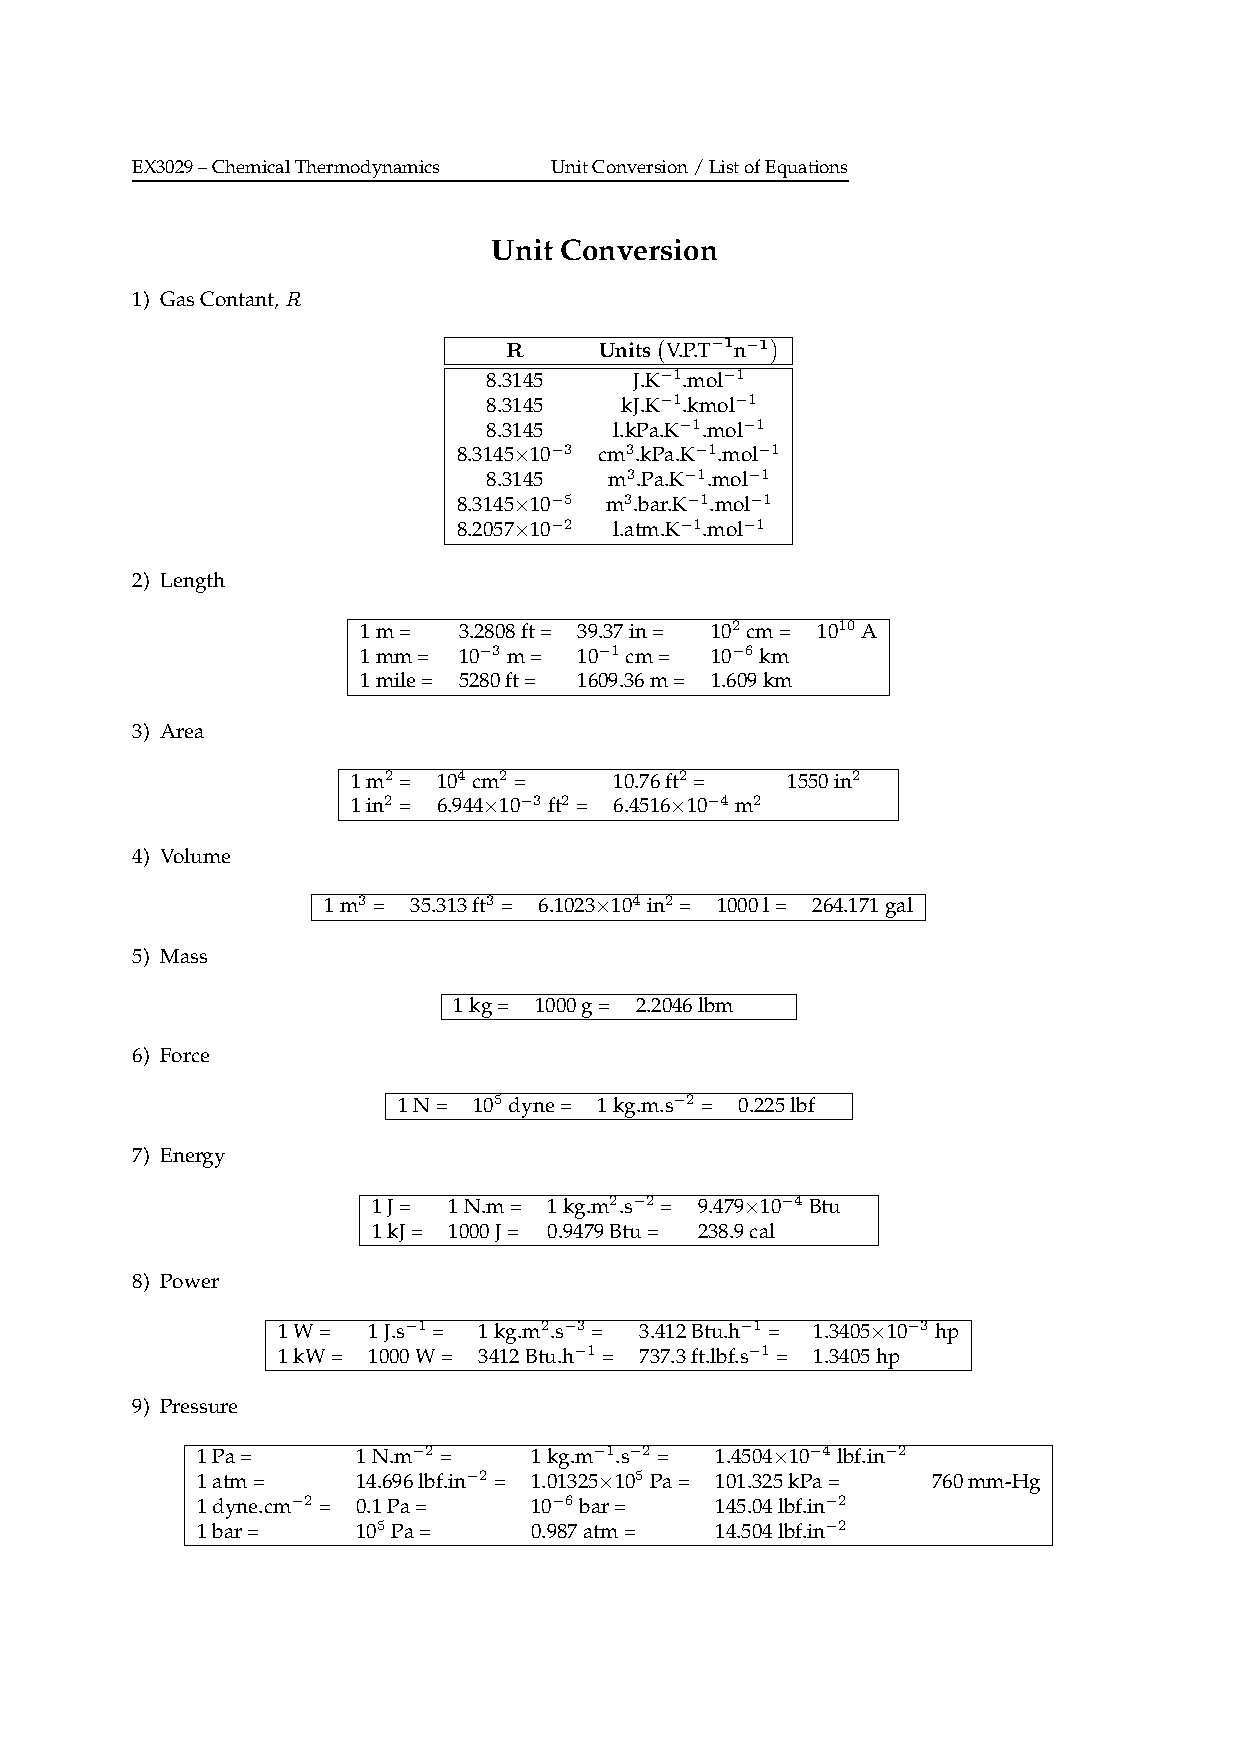
\includepdf[pages=-,fitpaper]{./Pics/EquationsList}
  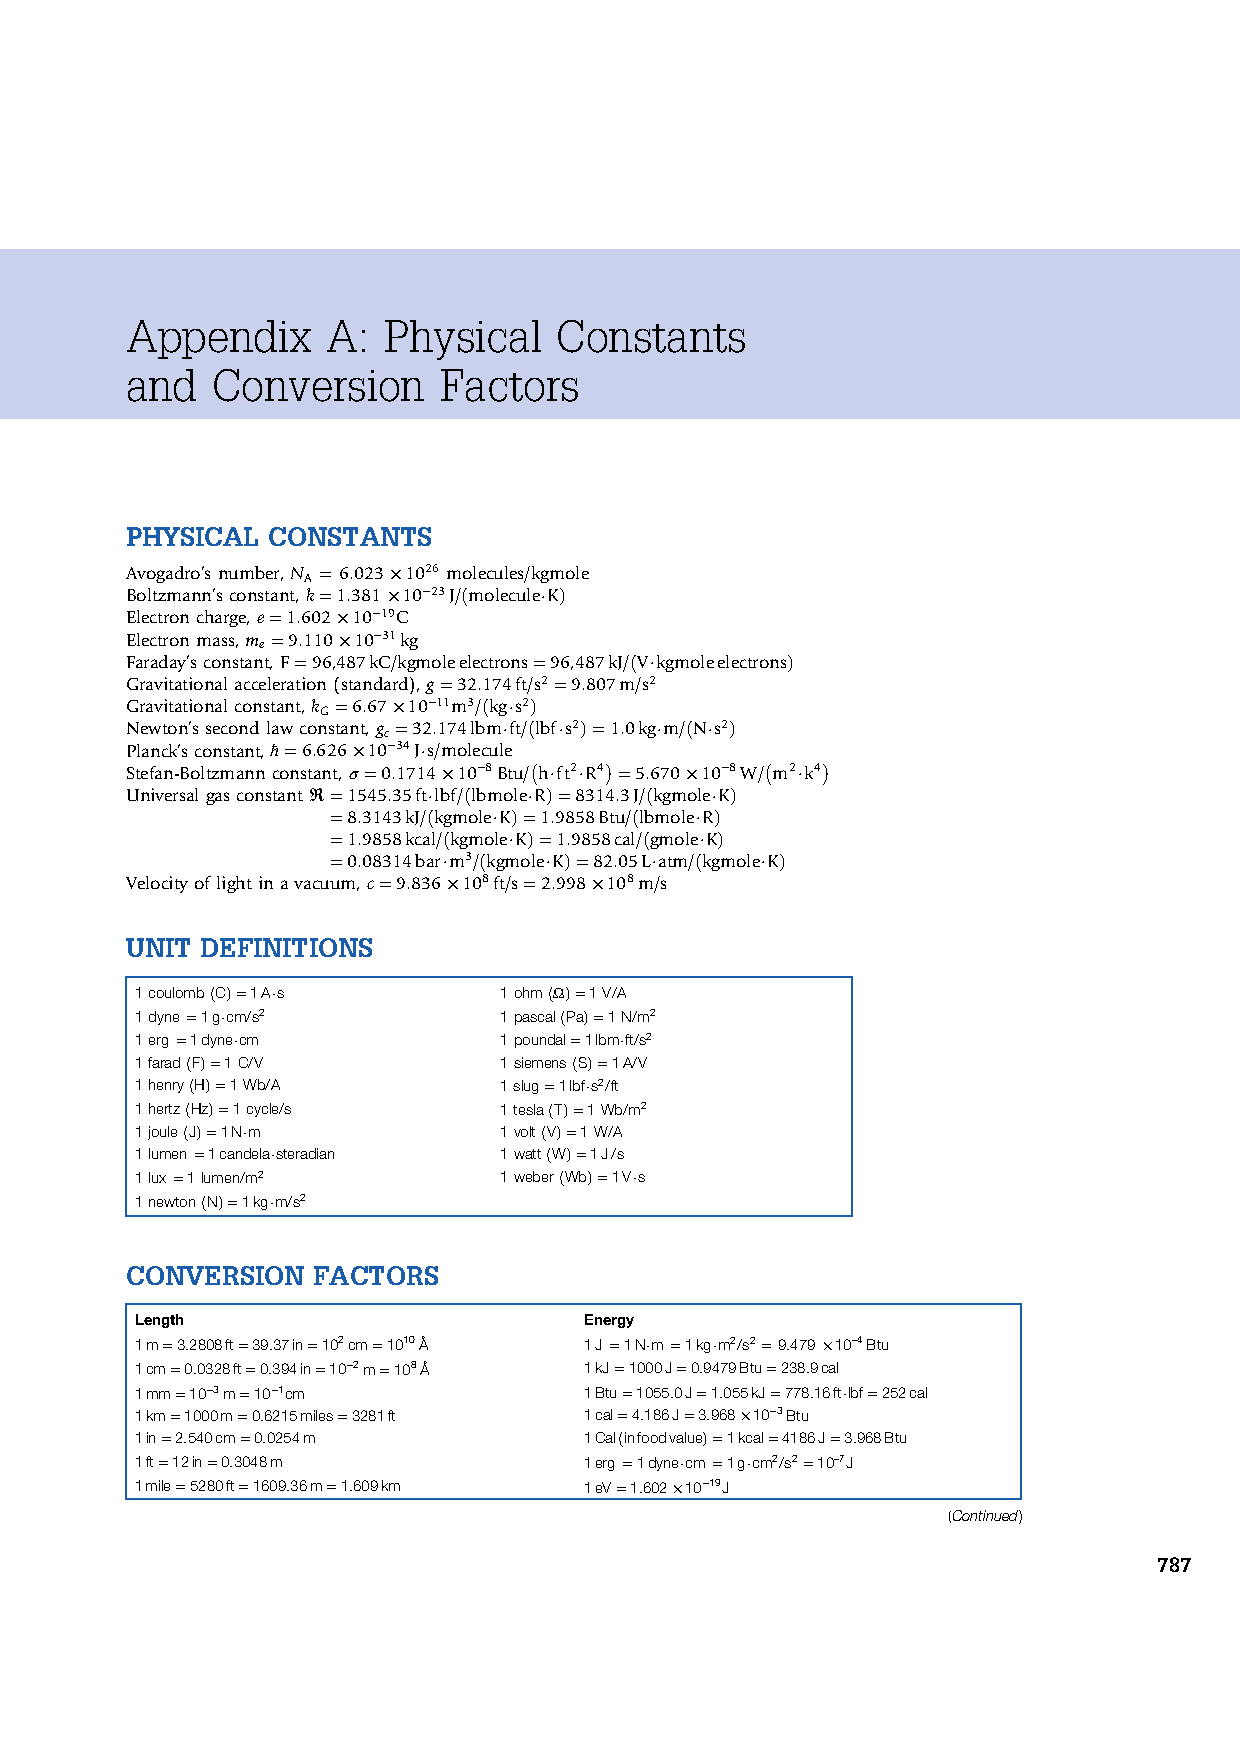
\includepdf[pages=-,fitpaper]{./Pics/ChemEng_UnitConv}
  %\includepdf[pages=-,fitpaper]{./Pics/ChemEng_NH3Tables}
}


\end{document}
